\documentclass[utf8]{article}

\usepackage[utf8]{inputenc}

\usepackage[parfill]{parskip}

\usepackage[T1]{fontenc}
\usepackage[french]{babel}
\usepackage{array,multirow,makecell}
\usepackage{longtable}
\usepackage{setspace}
\usepackage{makecell}
\setcellgapes{1pt}
\makegapedcells
\usepackage[table]{xcolor}
\renewcommand*{\emph}[1]{\textcolor{green}{#1}}
\newcolumntype{R}[1]{>{\raggedleft\arraybackslash }b{#1}}
\newcolumntype{L}[1]{>{\raggedright\arraybackslash }b{#1}}
\newcolumntype{C}[1]{>{\centering\arraybackslash }b{#1}}
\usepackage{amsmath}
\usepackage{amssymb}
\usepackage{amsfonts}
\usepackage{graphicx}
\usepackage{float}
\usepackage{algorithm}
\usepackage{algorithmicx}
\usepackage{algpseudocode}
\usepackage{fullpage}


% -----------------------------------------------------


\title{\\[3 cm]\Huge Software requirements document : \\[1 cm] L-type\\[7 cm]}
\author{ELKENZE Camelia\\[0,2 cm] BARBER Jeremy\\[0,2 cm] Latoundji Salim\\[0,2 cm] DEMIREL Helin\\[0,2 cm] ABDOUL-AZIZ Aïssa\\[0,2 cm] ADEGNON Kokou\\[0,2 cm] KINSOEN Alexandre\\[0,2 cm] VANNESTE Martin\\[0,2 cm] MASSIMETTI Mario  }
\date{20 novembre 2020}

\begin{document}
\tableofcontents

\newpage

% -----------------------------------------------------

\section{Introduction}
Bla bla \emph{bla}.

\subsection{But du projet}
L’objectif de ce projet est de réaliser un shoot them up multijoueur à scrolling vertical dans lequel un ou deux joueurs doivent parcourir plusieurs niveaux en détruisant les ennemis qui se présentent devant eux ainsi qu’en esquivant les salves de tir provoquées par ces derniers.
Les navires de guerre dirigés par les joueurs peuvent récupérer des bonus d’armement lâchés par leurs nombreux adversaires.

\subsection{Glossaire}
Shoot them up : "abattez-les tous", genre de jeu vidéo

\subsection{Historique}
Historique \emph{de notre travail}

\section{Besoins utilisateur}

\subsection{Besoins fonctionnels}

% ajoute de l'image

\begin{figure}[h!]
\centering
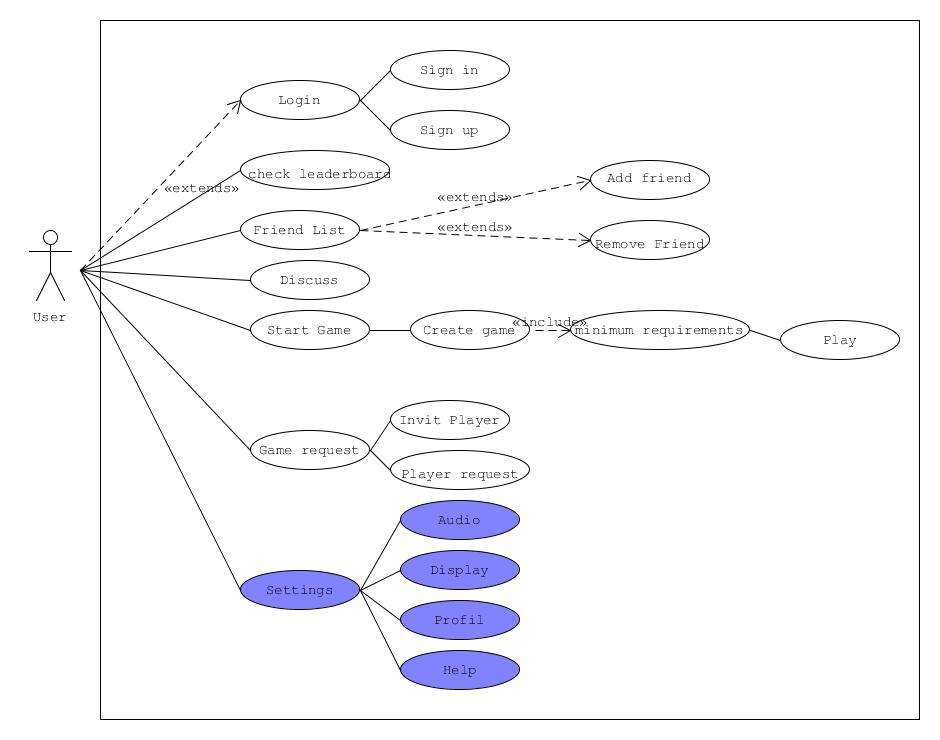
\includegraphics[width=10cm]{UserUseCase}
\caption{Diagramme de use case coté utilisateur}
\label{fig:UerUseCase}
\end{figure}

\subsubsection{Connexion}
L'utilisateur en lançant le programme arrive sur une page d’accueil qui l'invite à entrer son nom d'utilisateur et son mot de passe si ce dernier possède
deja un compte. S'il ne possède pas de compte il a la possibilité de créer un nouveau compte. Un pseudo et un mot de passe seront demandés tant que le format des entrées est incorrect et/ou que le pseudo n'est pas unique. Après s’être connecté l'utilisateur accède au menu principal.
\subsubsection{Menu principal}
\subsubsection{Création de partie}
\subsubsection{Connexion}
\subsubsection{Connexion}
\subsection{Besoins non fonctionnels}

\section{Besoins système}
\subsection{Besoins fonctionnels}
\subsubsection{Connexion}
\subsubsection{Menu principal}
\subsubsection{Création de partie}
\subsubsection{Connexion}
\subsubsection{Connexion}
\subsection{Besoins non fonctionnels}

\newpage
\section{Annexes}
\subsection{ Description du diagramme use case utilisateur}

\begin{center}
\begin{longtable}{|p{1,5cm}||p{3,5cm}|p{3,5cm}|p{3,5cm}|p{3,5cm}|}
\hline
\rowcolor{green}
USE CASE   &\center{Pré-conditions}   & \hfill Post-conditions \hfill\null & Cas Général & Cas exceptionnels\\
\hline
\hline
\textbf{Sign in}      & L'utilisateur doit être enregistré dans la base de données  & L'utilisateur est connecté à sa base de données et le menu principal est affiché & L'utilisateur déjà enregistré se connecte à son compte en tapant son nom d’utilisateur et mot de passe. Le système vérifie que les données soient correctes et donne accès au compte du client.  & Si l’identifiant ou le mot de passe sont incorrectes, le système affiche un message d'erreur a l'utilisateur. \\
\hline
\hline
\textbf{Sign up}     & L'utilisateur n'est pas présent dans la base de données   & Ajout d'un compte dans la base de données et affichage du menu principal & L'utilisateur crée un compte en introduisant un pseudo et un mdp  & Si les données entrées ne respectent pas le format requis ou que le nom d'utilisateur est déjà utilisé, un message d'erreur est affiché et l'utilisateur doit recommencer l'action jusqu'à ce que ce soit valide \\

\hline
\hline
\textbf{Create game}    & L'utilisateur doit être enregistré dans la base de données  & Possibilité de sauvegarder les options requises  & L'utilisateur peut lancer une partie après avoir rempli les conditions minimales  & Néant \\
\hline
\hline
\textbf{Invite player} & L'utilisateur doit être enregistré dans la base de données   & Etablissement de la connexion via le serveur entre l’hôte et l’invité. & Inviter un joueur avec son pseudo & Invitation via pseudo qui n’existe pas. \\
\hline
\hline
\textbf{Player request}  & Recevoir une invitation via le serveur.
L'utilisateur doit être enregistré dans la base de données   & Etablissement de la connexion via le serveur entre l’hôte et l’invité.  & Accepter/ Refuser une invitation de partie  & La connexion échouera si :
Accepter une invitation dont l'hôte n’est plus connecté.
Rejoindre un salon complet. \\
\hline
\hline
\textbf{Check Leaderboard}  & L'utilisateur doit être enregistré dans la base de données   & \hfill Néant  \hfill\null &Le joueur peut consulter le classement des meilleurs scores en envoyant une requête au serveur qui va lui renvoyer les informations  & Néant \\
\hline
\hline
\textbf{View friend list }   & L'utilisateur doit être enregistré dans la base de données   & Néant  & Consultation de liste d'ami dans la base de données. & Néant \\
\hline
\hline
\textbf{Chat}     & L'utilisateur doit être enregistré dans la base de données   & Le serveur effectue les liaisons entre les utilisateurs  & Envoyer et recevoir des messages avec n'importe quel pseudo.  & Néant \\
\hline
\hline
\textbf{Add friend}    & L'utilisateur doit être enregistré dans la base de données   & Si invitation acceptée, ajout d'amis dans la base de donnée (bidirectionnel).  & Entrer le pseudo d’un ami. Le système va rechercher dans la base de données si le pseudo existe et l’ajouter.  & Ajouter un ami qui n’existe pas (affiche une erreur).\\
\hline
\hline
\textbf{Delete friend}    & L'utilisateur doit être enregistré dans la base de données et avoir au moins un ami.   & Suppression d’amis(de la liste d’amis) de la base de données.  & Entrer le pseudo d’un ami. Le système va rechercher dans la base de données si le pseudo existe et le supprimer.  & Supprimer un ami qui n’existe pas (affiche une erreur). \\
\hline
\hline
\textbf{Settings}     & L'utilisateur doit être enregistré dans la base de données   & Mise à jour des changements  & L'utilisateur modifie des parametres de son profil de l'affichage ou du son  & Néant\\
\hline
\hline
\textbf{Ship’s controls}  & Charger une partie/créer une partie.   & Actualisation de l’état de jeu.  & Bouger, tirer recevoir des bonus.  & Néant\\
\hline
\hline
\textbf{Leave party}      & Être en train de jouer   & Retour au menu principal  & Le joueur arrête la partie en cours.  & Néant\\
\hline
\hline
\textbf{Help}      & Etre connecté   & Néant  & Les règles principales du jeu sont affichées au joueur & Néant\\
\hline
\hline
\textbf{Leave game}      & Etre connecté   & Fermeture du jeu  & L'utilisateur est connecté et veut quitter le jeu  & L'utilisateur est connecté et force sa sortie du jeu (CTRL+C, ...)\\
\hline
\end{longtable}
\end{center}


\end{document}
